% This file was created by matlab2tikz.
%
%The latest updates can be retrieved from
%  http://www.mathworks.com/matlabcentral/fileexchange/22022-matlab2tikz-matlab2tikz
%where you can also make suggestions and rate matlab2tikz.
%
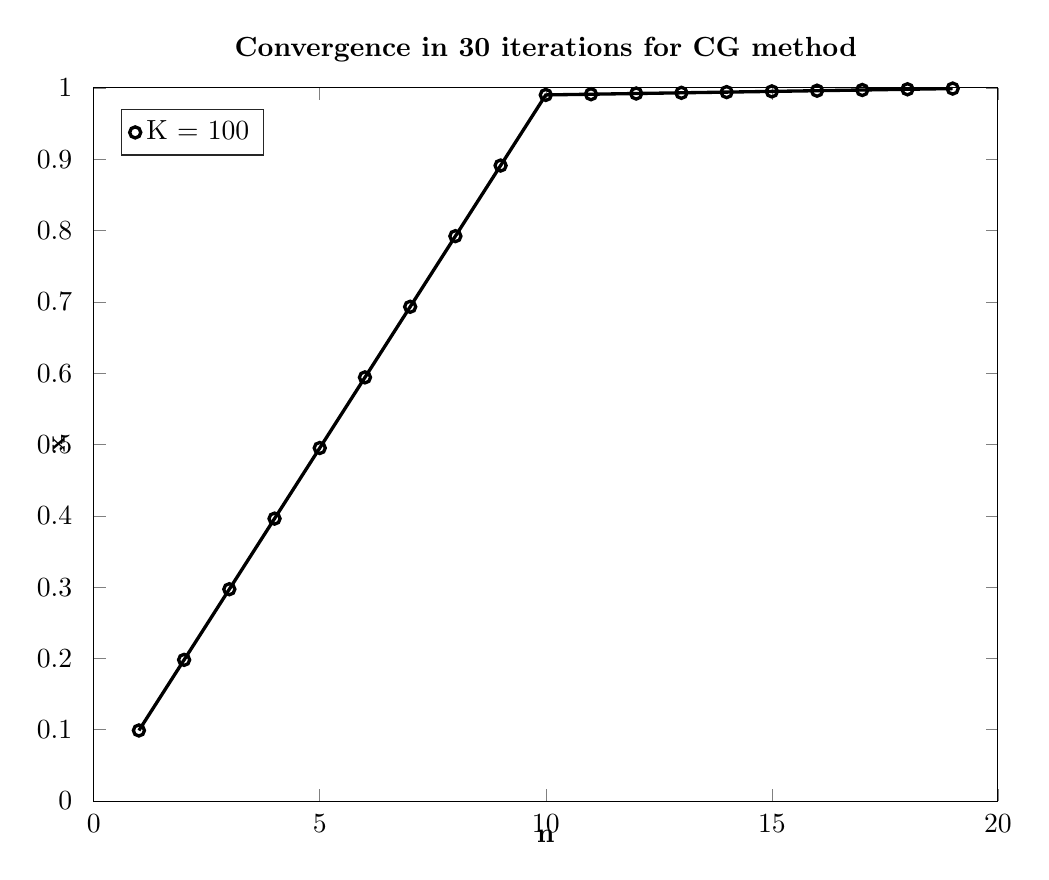
\begin{tikzpicture}

\begin{axis}[%
width=4.521in,
height=3.566in,
at={(0.758in,0.481in)},
scale only axis,
clip=false,
xmin=0,
xmax=20,
xtick={0,5,10,15,20},
xticklabels={\empty},
xlabel style={font=\bfseries},
xlabel={n},
ymin=0,
ymax=1,
ytick={0,0.1,0.2,0.3,0.4,0.5,0.6,0.7,0.8,0.9,1},
yticklabels={\empty},
ylabel style={font=\bfseries},
ylabel={x},
axis background/.style={fill=white},
title style={font=\bfseries},
title={Convergence in 30 iterations for CG method},
legend style={at={(0.03,0.97)},anchor=north west,legend cell align=left,align=left,draw=white!15!black}
]
\addplot [color=black,line width=1.2pt,only marks,mark=o,mark options={solid}]
  table[row sep=crcr]{%
1	0.0990099009900989\\
2	0.198019801980198\\
3	0.297029702970297\\
4	0.396039603960396\\
5	0.495049504950495\\
6	0.594059405940594\\
7	0.693069306930693\\
8	0.792079207920792\\
9	0.891089108910891\\
10	0.990099009900981\\
11	0.991089108910908\\
12	0.992079207920779\\
13	0.993069306930699\\
14	0.994059405940596\\
15	0.995049504950489\\
16	0.996039603960395\\
17	0.997029702970298\\
18	0.998019801980214\\
19	0.999009900990075\\
};
\addlegendentry{K = 100};

\addplot [color=black,solid,line width=1.2pt,forget plot]
  table[row sep=crcr]{%
1	0.0990099009900989\\
2	0.198019801980198\\
3	0.297029702970297\\
4	0.396039603960396\\
5	0.495049504950495\\
6	0.594059405940594\\
7	0.693069306930693\\
8	0.792079207920792\\
9	0.891089108910891\\
10	0.990099009900981\\
11	0.991089108910908\\
12	0.992079207920779\\
13	0.993069306930699\\
14	0.994059405940596\\
15	0.995049504950489\\
16	0.996039603960395\\
17	0.997029702970298\\
18	0.998019801980214\\
19	0.999009900990075\\
};
\node[align=center, text=black]
at (axis cs:0,-0.031) {$0$};
\node[align=center, text=black]
at (axis cs:5,-0.031) {$5$};
\node[align=center, text=black]
at (axis cs:10,-0.031) {$10$};
\node[align=center, text=black]
at (axis cs:15,-0.031) {$15$};
\node[align=center, text=black]
at (axis cs:20,-0.031) {$20$};
\node[left, align=right, text=black]
at (axis cs:-0.258,0) {$0$};
\node[left, align=right, text=black]
at (axis cs:-0.258,0.1) {$0.1$};
\node[left, align=right, text=black]
at (axis cs:-0.258,0.2) {$0.2$};
\node[left, align=right, text=black]
at (axis cs:-0.258,0.3) {$0.3$};
\node[left, align=right, text=black]
at (axis cs:-0.258,0.4) {$0.4$};
\node[left, align=right, text=black]
at (axis cs:-0.258,0.5) {$0.5$};
\node[left, align=right, text=black]
at (axis cs:-0.258,0.6) {$0.6$};
\node[left, align=right, text=black]
at (axis cs:-0.258,0.7) {$0.7$};
\node[left, align=right, text=black]
at (axis cs:-0.258,0.8) {$0.8$};
\node[left, align=right, text=black]
at (axis cs:-0.258,0.9) {$0.9$};
\node[left, align=right, text=black]
at (axis cs:-0.258,1) {$1$};
\end{axis}
\end{tikzpicture}%